\section{Introduction}

% \textbf{Why should I care?}

% Large language models can do cool stuff, including few-shot cool stuff and adaptation for even more cool stuff. Large language models recently became publicly available: bloom-176b, opt-175b, maybe yalm-100b.
In recent years, the NLP community has found that pretrained language models can solve many practical tasks, through either fine-tuning~\citep{gpt} or simple prompting~\citep{gpt3}. Furthermore, performance tends to improve as scale increases~\citep{gpt2, kaplan2020scaling}. Following this trend, modern language models often have hundreds of billions of parameters~\citep{gpt3,gopher,pangua,hyperclova}\nocite{switch,jurrasic,Lepikhin2020GShardSG,glam}. Several research groups released pretrained LLMs with over 100B parameters~\citep{opt,yalm,zeng2020glm}\nocite{gpt,gpt-neox-20b}. Most recently, the BigScience project has released BLOOM, a 176 billion parameter model supporting 46 natural and 13 programming languages~\citep{bloom}.

%Inferencing a pre-trained BLOOM requires 300-400GB of combined GPU memory, this is only possible on super high-end servers or multi-node clusters. You et al. cannot run language models on Your et al. computer. This slows down scientific progress in the area.

While the public availability of 100B+ parameter models makes them easier to access, they remain difficult to use for the majority of researchers and practitioners due to memory and computational costs. For instance, OPT-175B and BLOOM-176B need over 350 GB accelerator memory for inference and significantly more for fine-tuning. As a result, these LLMs usually require multiple high-end GPUs or multi-node clusters\nocite{megatron2} to be run. Both of these options are extremely expensive, which limits research and potential applications of LLMs.

% \paragraph{Option 1: running locally with offloading.}{Explain base principles of offloading, cite L2L, DS-Offload (anything else?).}
% Offloading is only efficient if you can form a huge batch and wait for several minutes. Some practical applications need to respond quickly. E.g., chat bots, translation services, search engines, any web service that interacts with the user. If you inference BLOOM with RAM offloading, you get 3 steps per minute on PCIE-gen3-x16.
% RAM offloading requires server hardware. A low-end GPU server with 512GB RAM still costs >\$10k. If you offload to SSD / HDD instead of RAM, you get one generation step per minute (latest nvme) or step per 30 minutes (sata ssd).

%To alleviate the mounting costs, NLP practitioners came up with several strategies to run LLMs more affordably.
Several recent works aim to democratize LLMs
by ``offloading'' model parameters to slower but cheaper memory (RAM or SSD), then running them on the accelerator layer by layer~\citep{l2l,zerooffload}\nocite{accelerate}.
%With offloading, one can run LLMs on cheaper systems, e.g. single-GPU servers with large amounts of RAM.
% However, using this technique comes at a cost of reduced performance, as one needs to transfer gigabytes worth of parameters every time a layer is used. As a result, it is only efficient only ``offline'' \textit{large-batch} inference.%, where one can load a layer once and process many parallel sequences.
This method allows running LLMs with a single low-end accelerator by loading parameters from RAM justin-time for each forward pass.
Offloading can be efficient for processing many tokens in parallel, but it has inherently high latency: for example, generating one token at a time with BLOOM-176B takes at least \textit{5.5~seconds} for the fastest RAM offloading setup and 22~seconds for the fastest SSD offloading. In addition, many computers do not have enough RAM to offload 175B parameters.

\begin{figure*}[t]
    \centering
    \vspace{-16pt}
    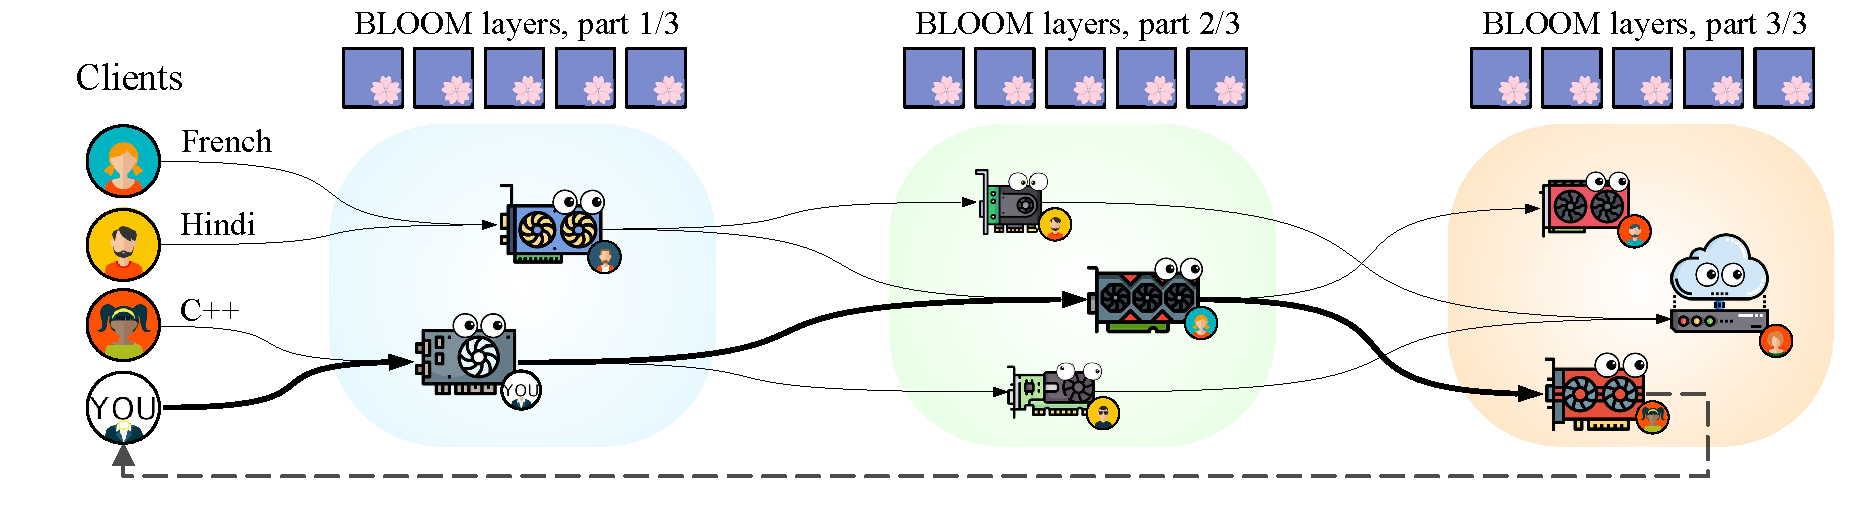
\includegraphics[width=\linewidth]{resources/bloom_swarm_v9a.pdf}
    \vspace{-16pt}
    \caption{An overview of \textsc{Petals}. Some participants (\textit{clients}) want to use a pretrained language model to solve various tasks involving processing texts in natural (e.g., French, Hindi) or programming (e.g., C++) languages. They do it with help of other participants (\textit{servers}), who hold various subsets of model layers on their GPUs. Each client chooses a sequence of servers so that it performs an inference or fine-tuning step in the least amount of time.}
    \label{fig:overview}
    \vspace{-12pt}
\end{figure*}

% \textbf{Existing strategies for running large models}
% \textbf{Option 2: hosted APIs:} describe the general idea of how APIs works. Cite openai, jurassic, forefront. APIs are the easiest way to use large LMs, as long as your use case is compatible. 
%APIs are not flexible. It's impossible to access internals (e.g. hidden states) unless API was explicitly designed to let you do that. If you extend/improve the model, it's hard to update an existing API unless you own it.
Another way to make LLMs more accessible is through public inference APIs, where one party hosts the model and lets others query it over the Internet~\citep{openai-api,jurrasic,forefront}. Since most of the engineering work is done by the API owner, this is a relatively user-friendly option.
However, APIs are often not flexible enough for research use: there is no way to change the model control flow or access internal states. On top of that, current API pricing can make some research projects prohibitively expensive~\citep{tfew}.

% \textbf{We propose Running large models collaboratively.} Instead running the whole model, a user would only host a subset of model layers - and rely on each other to run the full model. This strategy would be infeasible for few-billion models, but becomes efficient around 100B+ parameters (cite). 
In this work, we explore an alternative strategy inspired by crowdsourced distributed training of neural networks from scratch~\citep{hivemind_dmoe}. We introduce \textsc{Petals}, a platform that allows multiple users to collaborate and perform inference and fine-tuning of large language models over the Internet.
Each participant runs a server, a client or both. A server hosts a subset of model layers (typically, Transformer blocks) and handles requests from clients.
A client can form a chain of pipeline-parallel consecutive servers to run the inference of the entire model (Section~\ref{sect:design_inference}).
Aside from inference, participants can fine-tune the model through parameter-efficient training methods like adapters \citep{houlsby2019parameter} or prompt tuning \citep{ptune-lester} or by training entire layers (Section~\ref{sect:design_training}). Once trained, submodules can be shared on a model hub (Section~\ref{sect:design_ecosystem}), where others can use them for inference or further training.
% This design is based on the observation that, for a sufficiently large model, sending $O(\texttt{hidden\_size})$ activations over the network becomes cheaper than offloading $O(\texttt{hidden\_size}^2)$ parameters~\citep{swarm, activation-compression-with-guarantees}.
We demonstrate that existing 100B+ models can run efficiently in this setting with the help of several optimizations: dynamic quantization, prioritizing low-latency connections, and load balancing between servers (Section~\ref{sect:internals}).

% We describe the optimizations that make this system practical: using quantization to fit on low-end devices, prioritizing ``nearby'' servers for low latency, and assigning optimal layers to servers.



% \textbf{The rest of the paper is organized as follows:}
% \begin{itemize}
%     \vspace{-5px}\item Section 2: describe the system and go through main use cases
%     \vspace{-5px}\item Section 3: explain the internals, measure performance, eval model quality
%     \item Section 4: discuss how to facilitate sharing; discuss how to incentivize peers
% \end{itemize}
% FILLER TEXT TO ACCOUNT FOR REQUIRED SPACE \lipsum[4]
